%\documentclass[t,10pt]{beamer}
\documentclass[t,handout]{beamer}

\usepackage{graphicx}
\usepackage{epsfig}
\usepackage{psfrag}
\usepackage[english]{babel}
\usepackage{xcolor}
\usepackage{natbib}
\usepackage{booktabs}
\usepackage{listings}

% Font settings:
\usepackage[T1]{fontenc}
\usepackage{mathptmx}
\usepackage[scaled]{helvet}
\usepackage{courier}
\usepackage{microtype}



%Mathematics packages
\usepackage{amsmath}
\usepackage{mathrsfs}
\usepackage{amsfonts}
\usepackage{enumerate}

\graphicspath{{./images/}} % Figures path - used in graphicx

\selectcolormodel{cmyk}

\mode<presentation>

%THEMES - Please refer to these chapters in the beamer documentation.
% Presentation themes : Chapter 15
% Color themes : Chapter 17
% Font themes : Chapter 18
\usetheme{Pittsburgh}
\usecolortheme{orchid}
\usefonttheme{default}

\setbeamertemplate{bibliography item}[text]
\setbeamercovered{transparent=7}

%---------------------------Title frame definition------------------------------------- 

\title{Towards Robust Trust in Software Defined Networks}
\author [Chris]{Christopher C. Lamb}
\institute[University of New Mexico]{
\inst {}Department of Electrical and Computer Engineering\\
University of New Mexico}
\date{December 7, 2014}
\titlegraphic{
\begin{figure} 

\includegraphics[width = 7cm]{UNM}
\end{figure}}

% Delete this, if you do not want the table of contents to pop up at
% the beginning of each subsection:
%\AtBeginSubsection[]
%{
%  \begin{frame}<beamer>
%    \frametitle{Outline}
%     \tableofcontents[currentsection,currentsubsection]
%  \end{frame}
%}

\begin{document}

\begin{frame}
\titlepage
\end{frame}

% This command will make the logo appear on all frames excluding the title frame.
\logo {
\includegraphics[width = 2.5cm]{UNM}}

\begin{frame}\frametitle{Networks in the Bad Old Days}
\begin{figure}[!t]
\centering
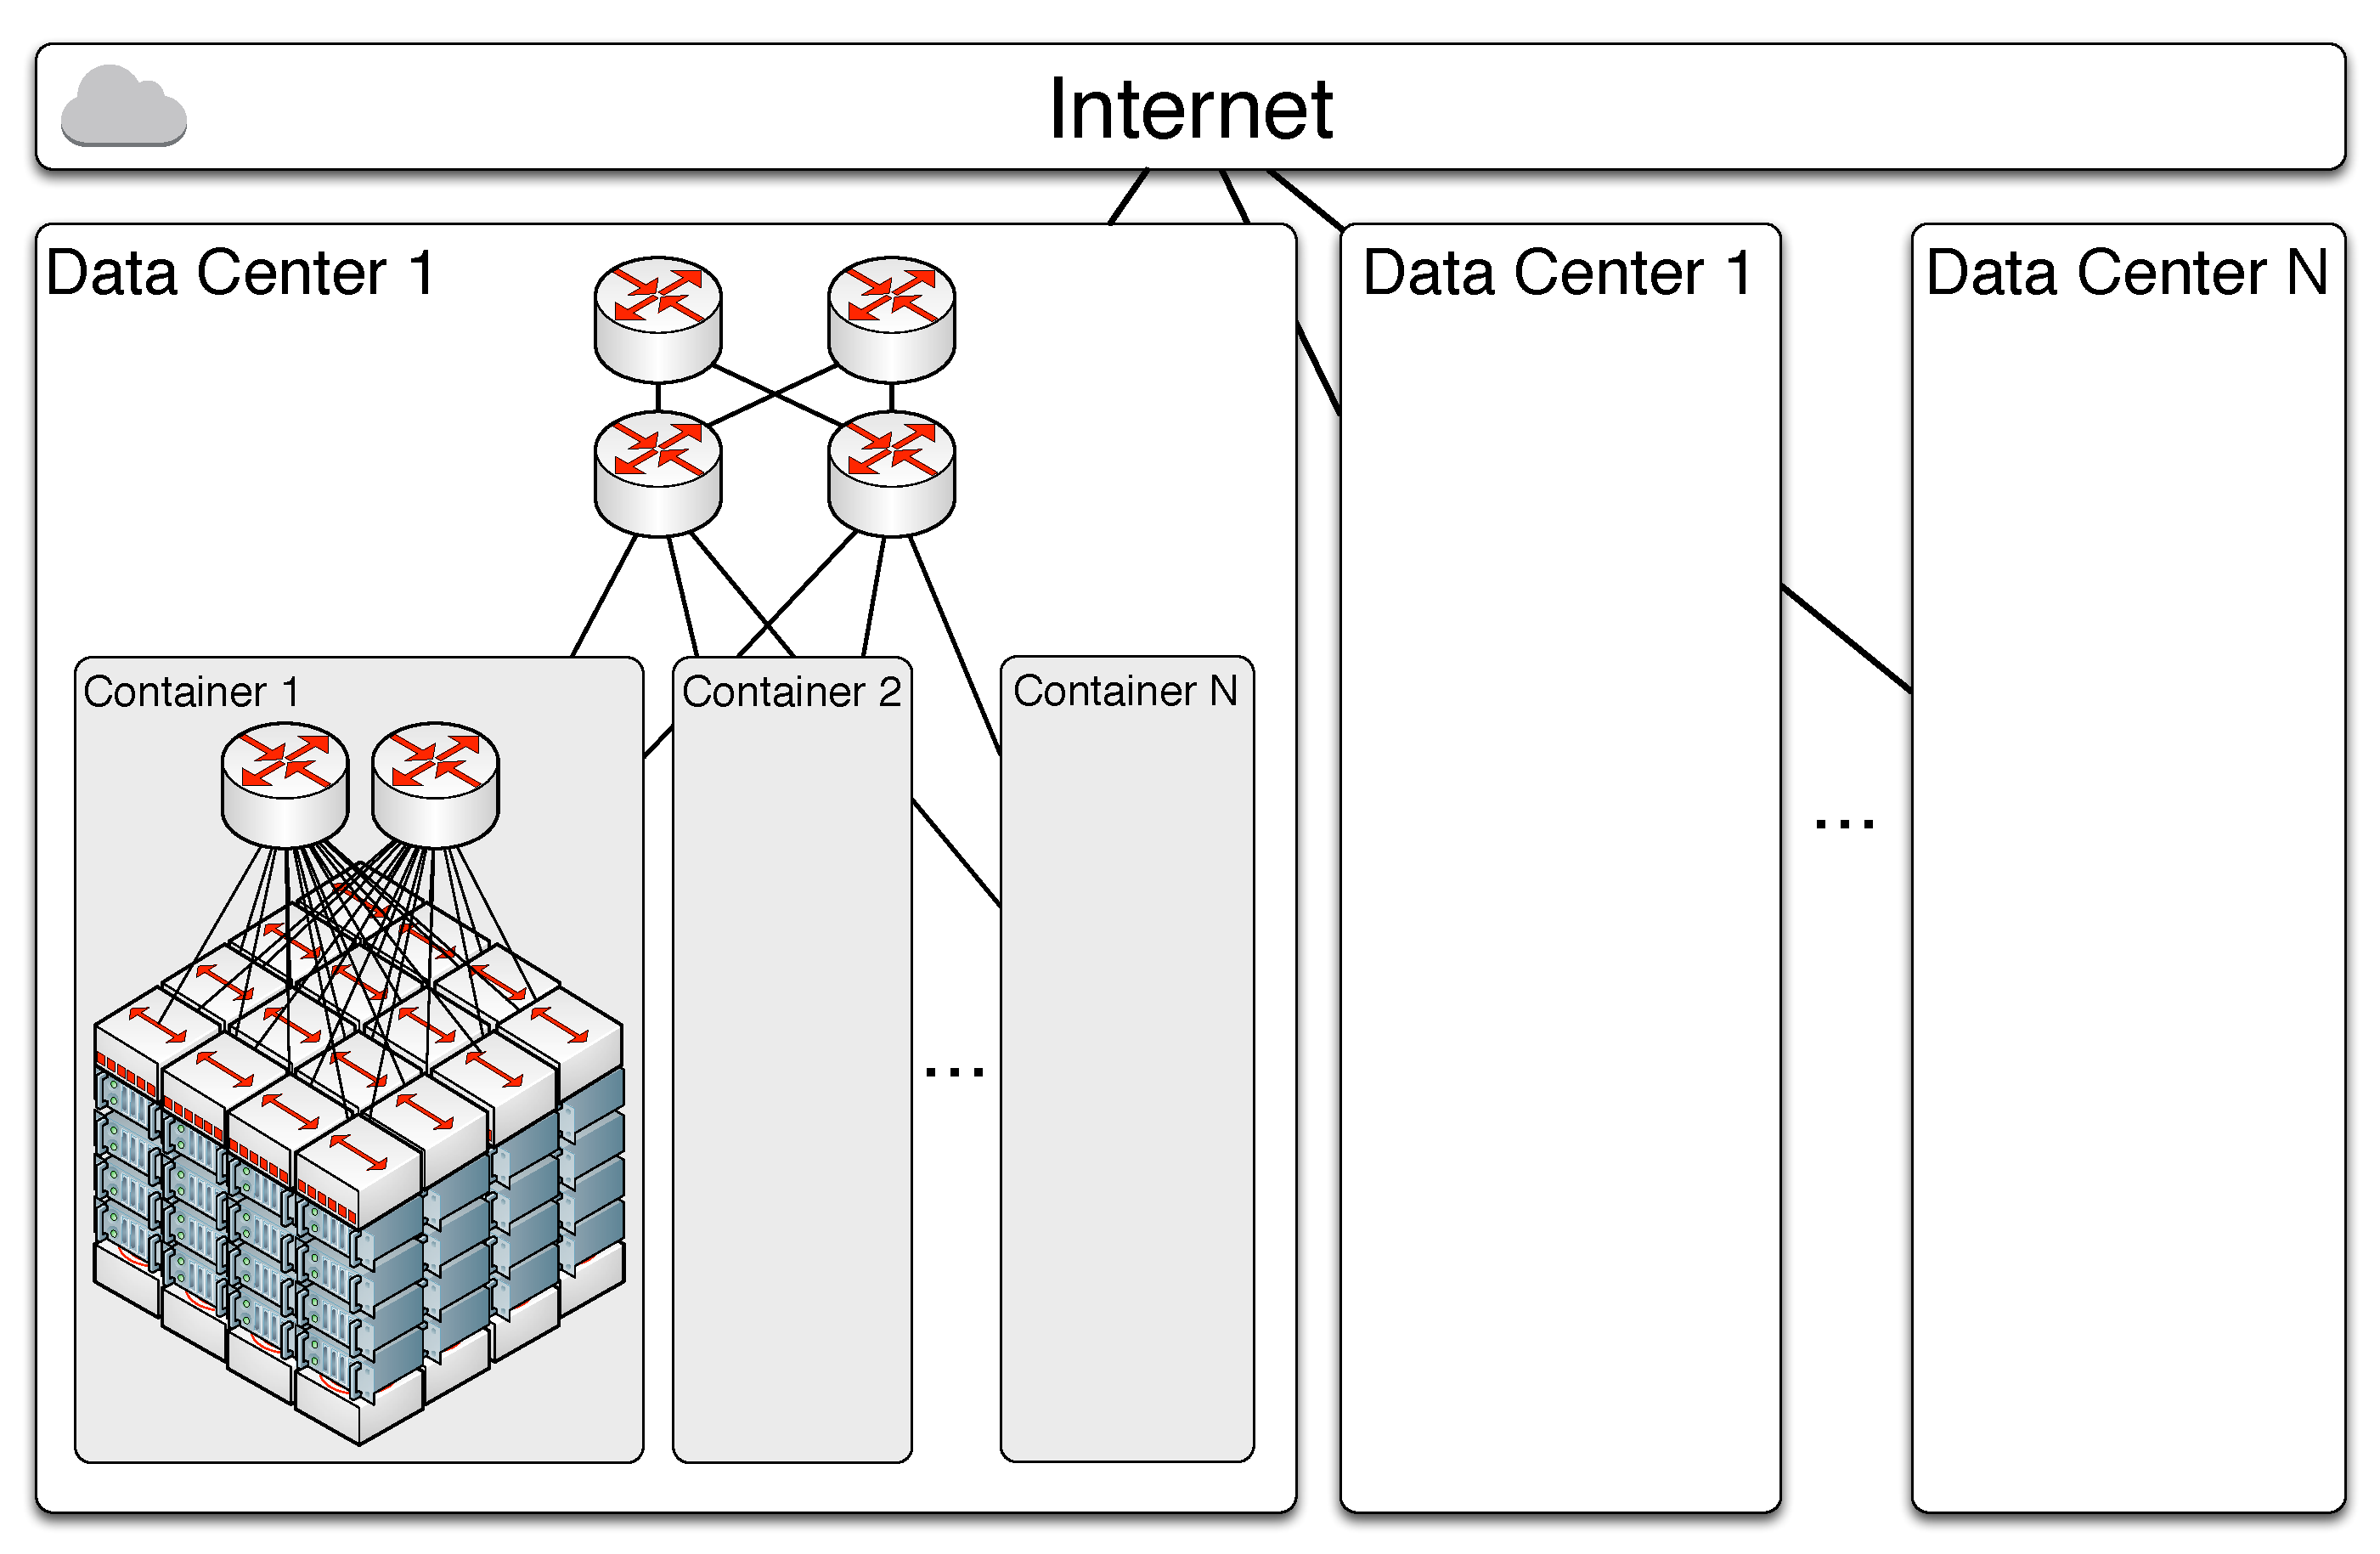
\includegraphics[height=2.75in]{lrg-network}
%\caption{Hierarchical Results from Comcast}
\end{figure}
\end{frame}

\begin{frame}
\frametitle{The Brave New World!}
\begin{figure}[!t]
\centering
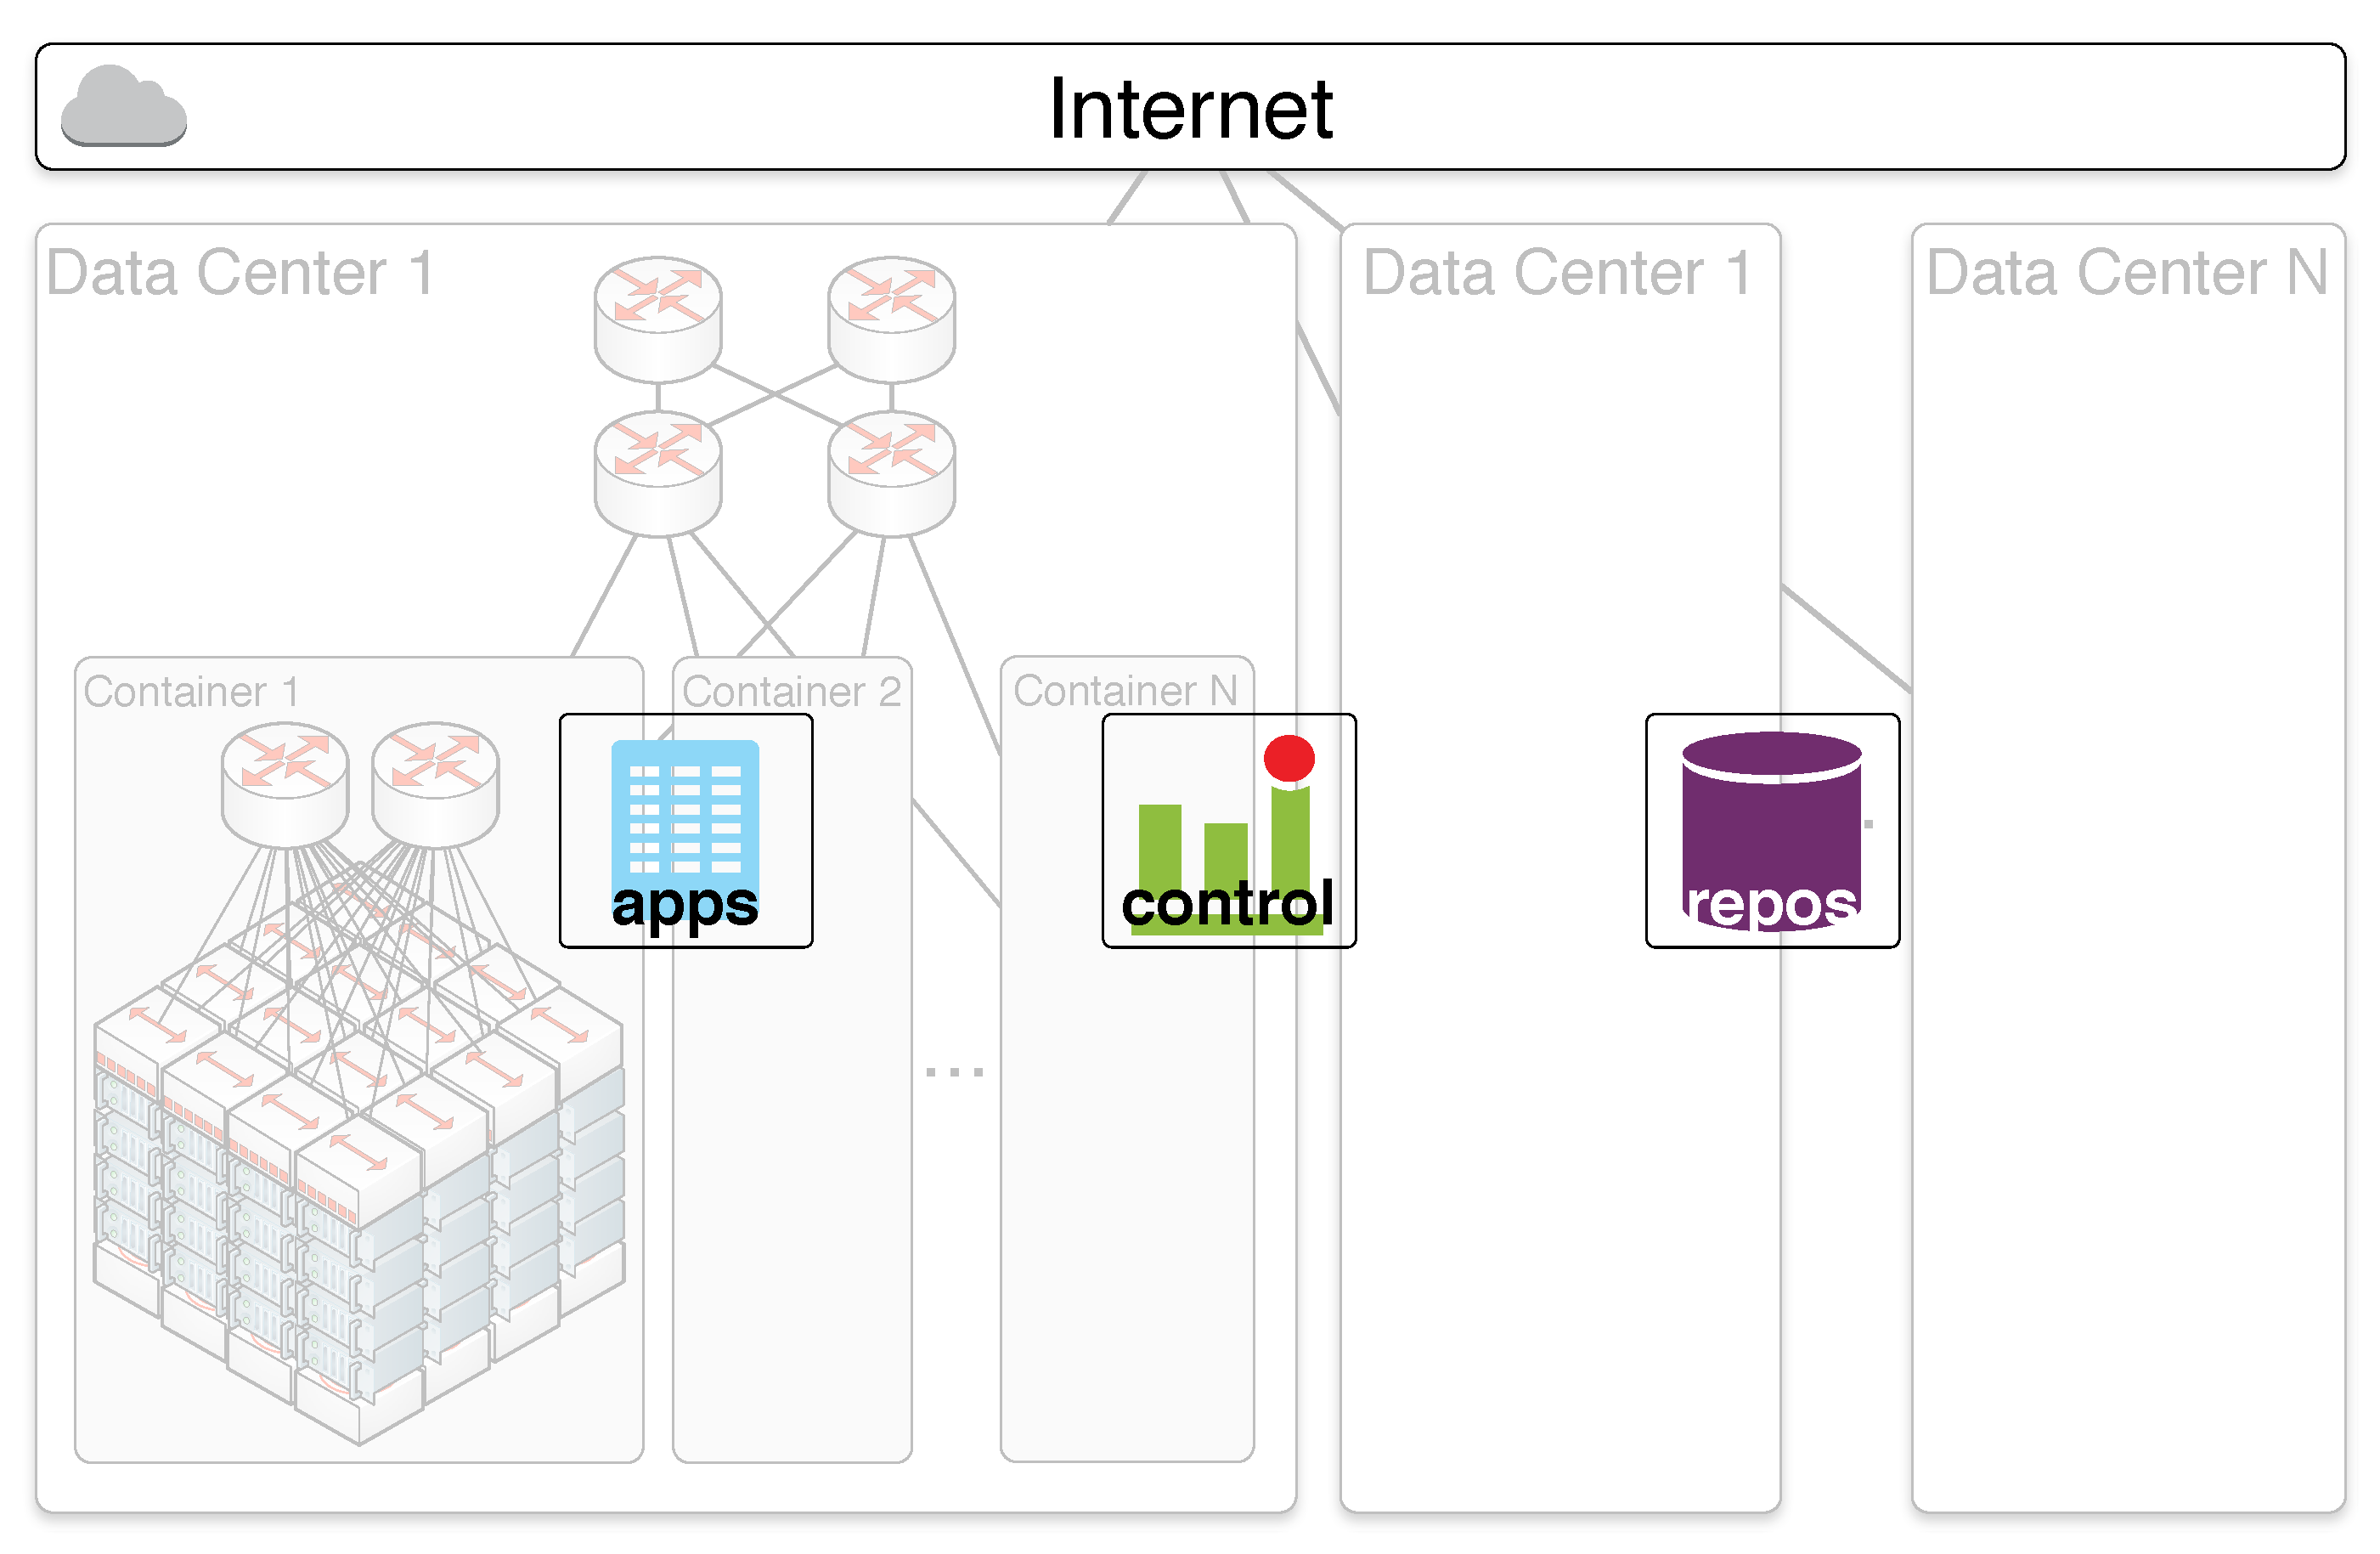
\includegraphics[height=2.75in]{lrg-network-sdn}
\end{figure}
\end{frame}

\begin{frame}
\frametitle{Brave New Implications}
\begin{columns}[T]
\column{.5\textwidth}
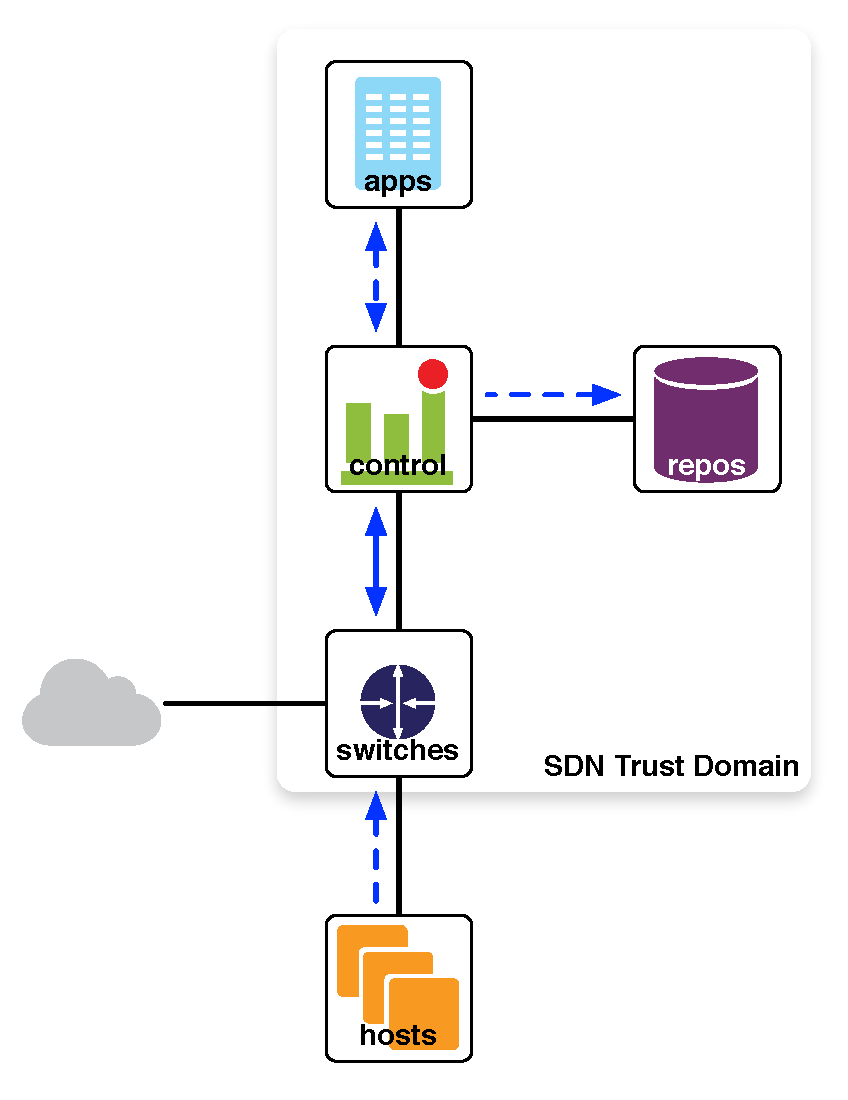
\includegraphics[height=2.75in]{reference-model}
\column{.5\textwidth}
\begin{beamerboxesrounded}[shadow]{Unintended Results of SDN}
Moving to centralized management has profound implications.
\begin{itemize}
\item Trust loci provides greater spoofing opportunities
\item Smaller number of involved systems refines target space
\item Trust concentration leads to larger attack surface
\item Single compromise can have outsized effects
\end{itemize}
\end{beamerboxesrounded}
\end{columns}
\end{frame}

%\begin{frame}
%\frametitle{Brave New Implications}
%\begin{columns}[T]
%\column{.5\textwidth}
%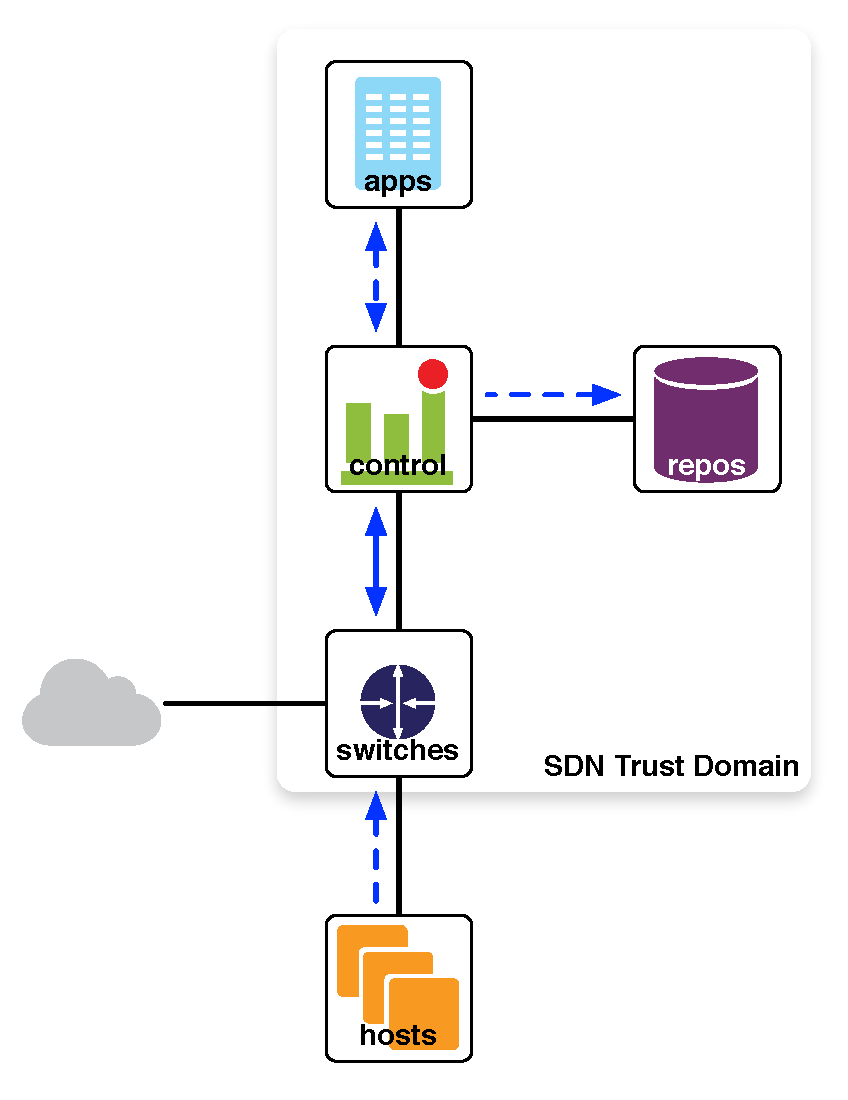
\includegraphics[height=2.75in]{reference-model}
%\column{.5\textwidth}
%\begin{beamerboxesrounded}[shadow]{Unintended Results of SDN}
%Moving to centralized management has profound implications.
%\begin{itemize}
%\item Trust loci provides greater spoofing opportunities
%\item Smaller number of involved systems refines target space
%\item Trust concentration leads to larger attack surface
%\item Single compromise can have outsized effects
%\end{itemize}
%\end{beamerboxesrounded}
%\end{columns}
%\end{frame}

\begin{frame}
\frametitle{host $\Longleftrightarrow$ switch}
\begin{columns}[T]
\column{.5\textwidth}
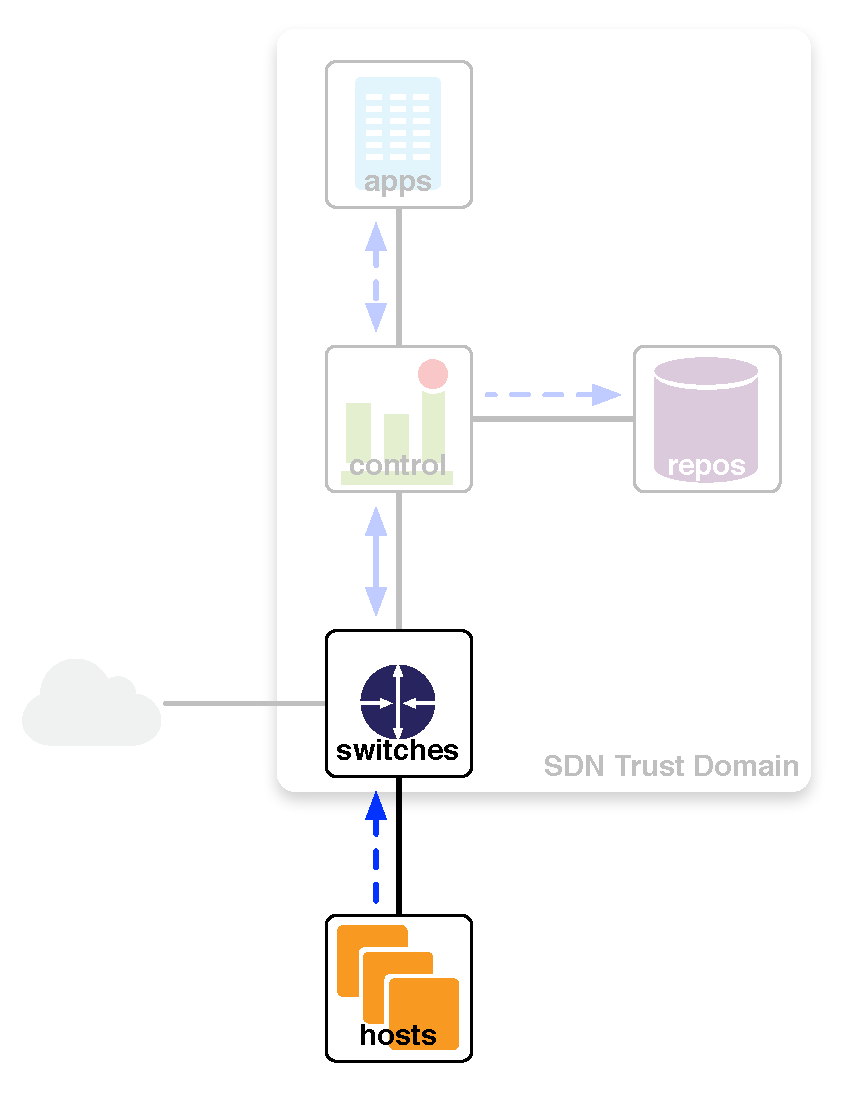
\includegraphics[height=2.75in]{ra-h-sw}
\column{.5\textwidth}
(In the following slides, {\color{red} red} is very important, {\color{orange} orange} less so, and {\color{green} green} even less).
\\~\\
\begin{beamerboxesrounded}[shadow]{}
\begin{itemize}
\item {\color{orange} Confidentiality not critical}
\item {\color{red} Integrity vital}
\item {\color{orange} Availability expected} 
\item {\color{green} Non-repudiation nice under certain circumstances}
\item {\color{green} Authentication likewise handy at times}
\end{itemize}
\end{beamerboxesrounded}
\end{columns}
\end{frame}

\begin{frame}
\frametitle{switch $\Longleftrightarrow$  controller}
\begin{columns}[T]
\column{.5\textwidth}
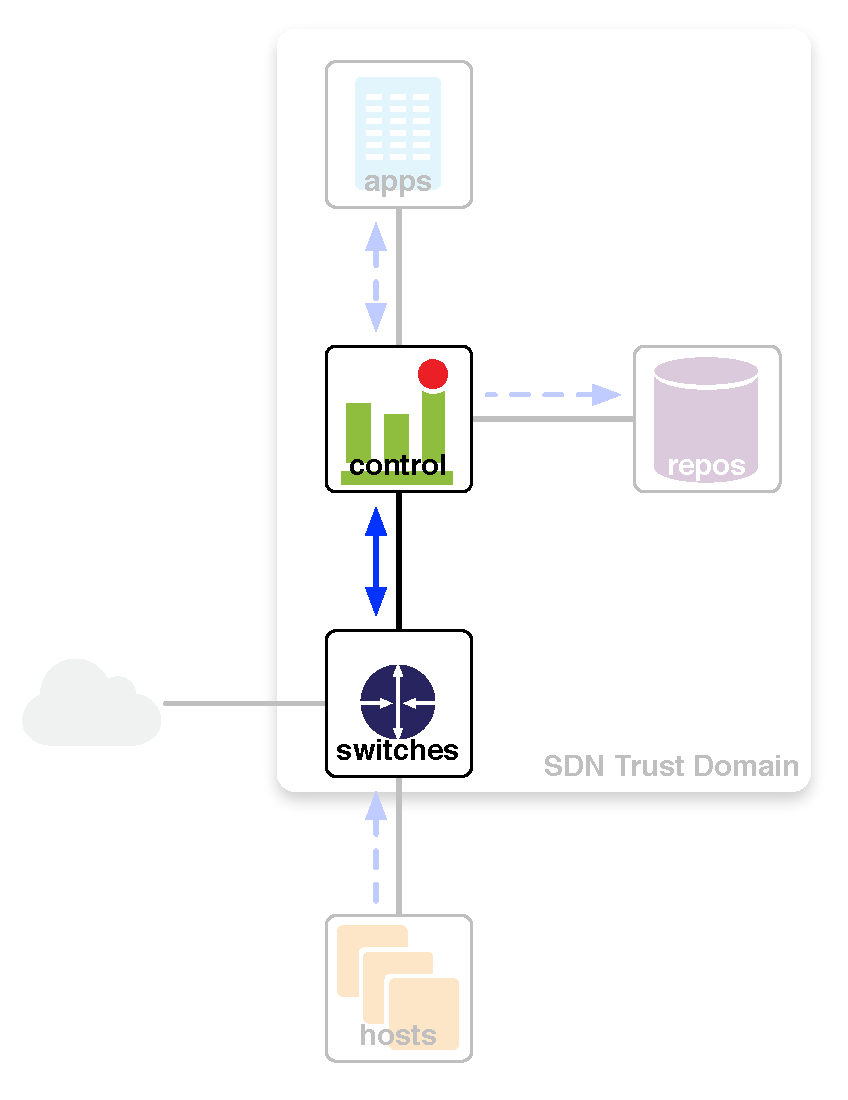
\includegraphics[height=2.75in]{ra-sw-c}
\column{.5\textwidth}
\begin{beamerboxesrounded}[shadow]{}
\begin{itemize}
\item {\color{orange} Confidentiality only important in some edge cases}
\item {\color{red} Integrity again vital}
\item {\color{red} Availability paramount} 
\item {\color{orange} Non-repudiation perhaps more important}
\item {\color{red} Authentication of controllers important}
\end{itemize}
\end{beamerboxesrounded}
\end{columns}
\end{frame}

\begin{frame}
\frametitle{controller $\Longleftrightarrow$ repository}
\begin{columns}[T]
\column{.5\textwidth}
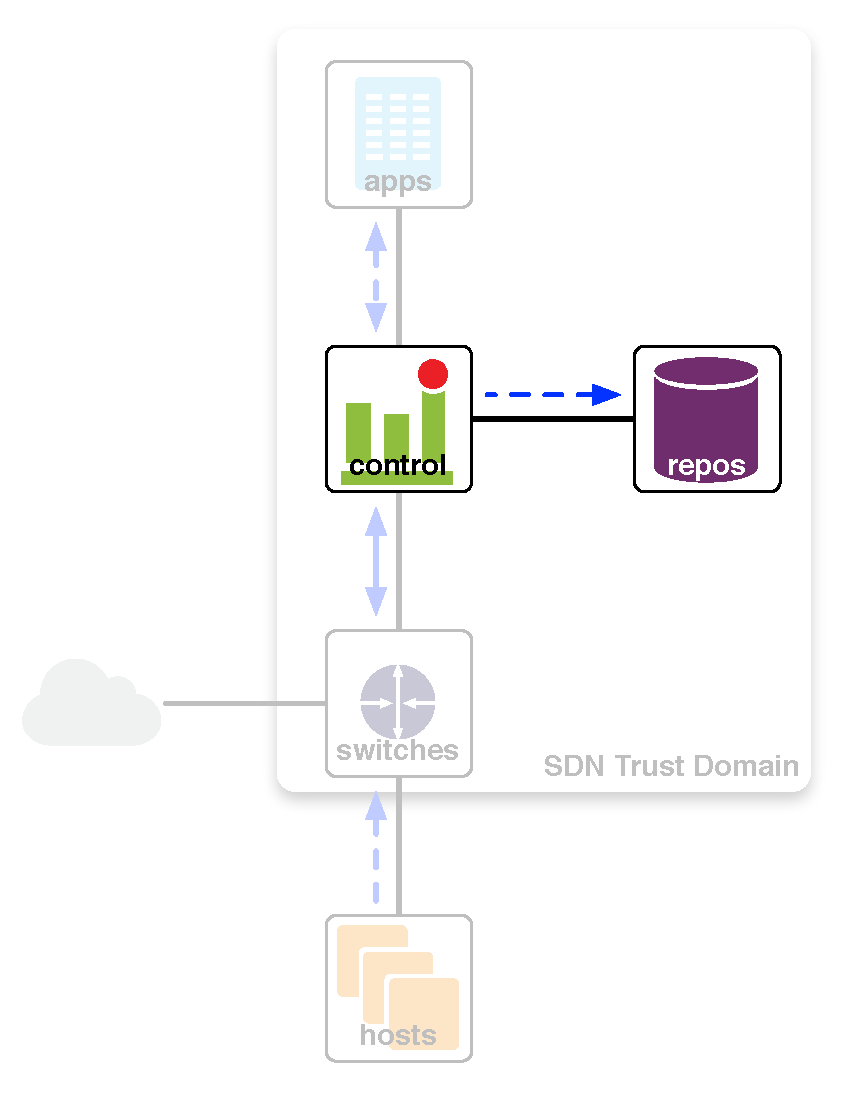
\includegraphics[height=2.75in]{ra-c-r}
\column{.5\textwidth}
\begin{beamerboxesrounded}[shadow]{}
\begin{itemize}
\item {\color{orange} Confidentiality not always vital}
\item {\color{red} Integrity important, as usual}
\item {\color{green} Availability not vital} 
\item {\color{green} Non-repudiation less important for core control plane functions}
\item {\color{red} Authentication of repositories important}
\end{itemize}
\end{beamerboxesrounded}
\end{columns}
\end{frame}

\begin{frame}
\frametitle{controller $\Longleftrightarrow$  application}
\begin{columns}[T]
\column{.5\textwidth}
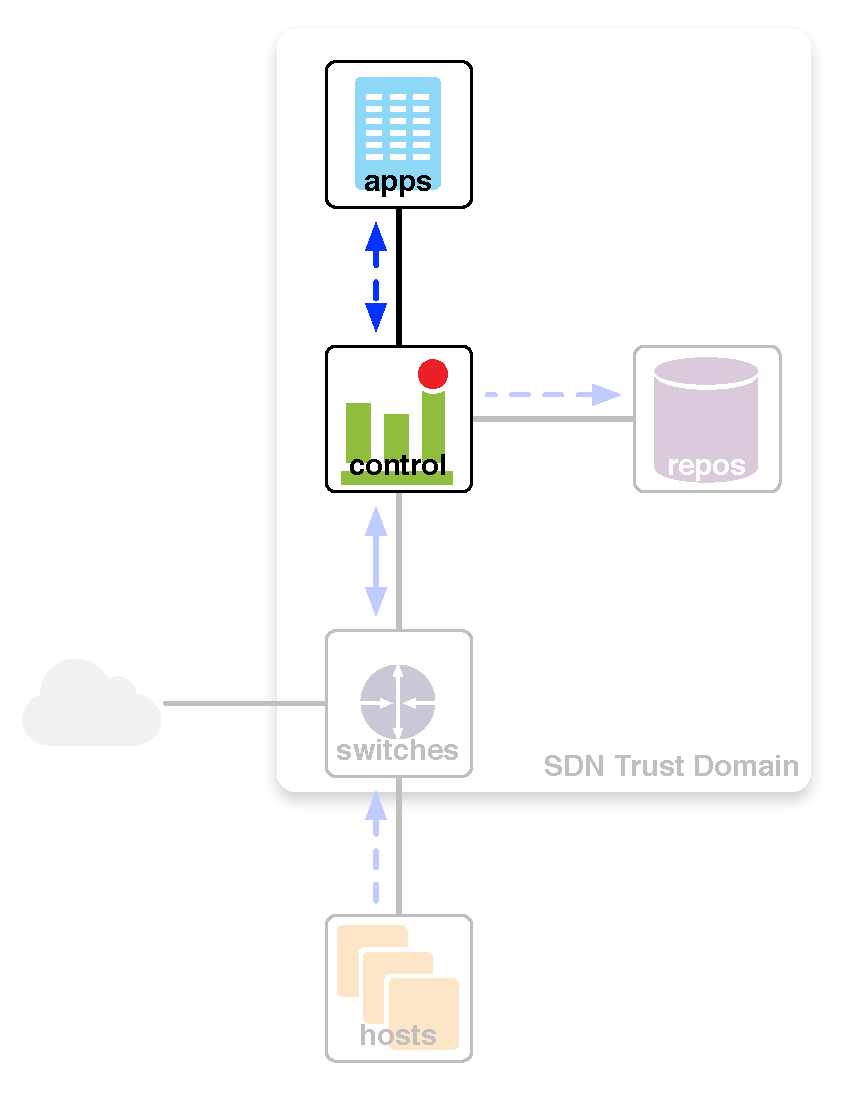
\includegraphics[height=2.75in]{ra-c-a}
\column{.5\textwidth}
\begin{beamerboxesrounded}[shadow]{}
\begin{itemize}
\item {\color{orange} Confidentiality based on application}
\item {\color{red} Integrity important, as usual}
\item {\color{green} Availability not vital} 
\item {\color{green} Non-repudiation needs again based on application}
\item {\color{red} Authentication of certain applications important}
\end{itemize}
\end{beamerboxesrounded}
\end{columns}
\end{frame}

\begin{frame}
\frametitle{Attribute Commonality}
\begin{columns}[T]
\column{.5\textwidth}
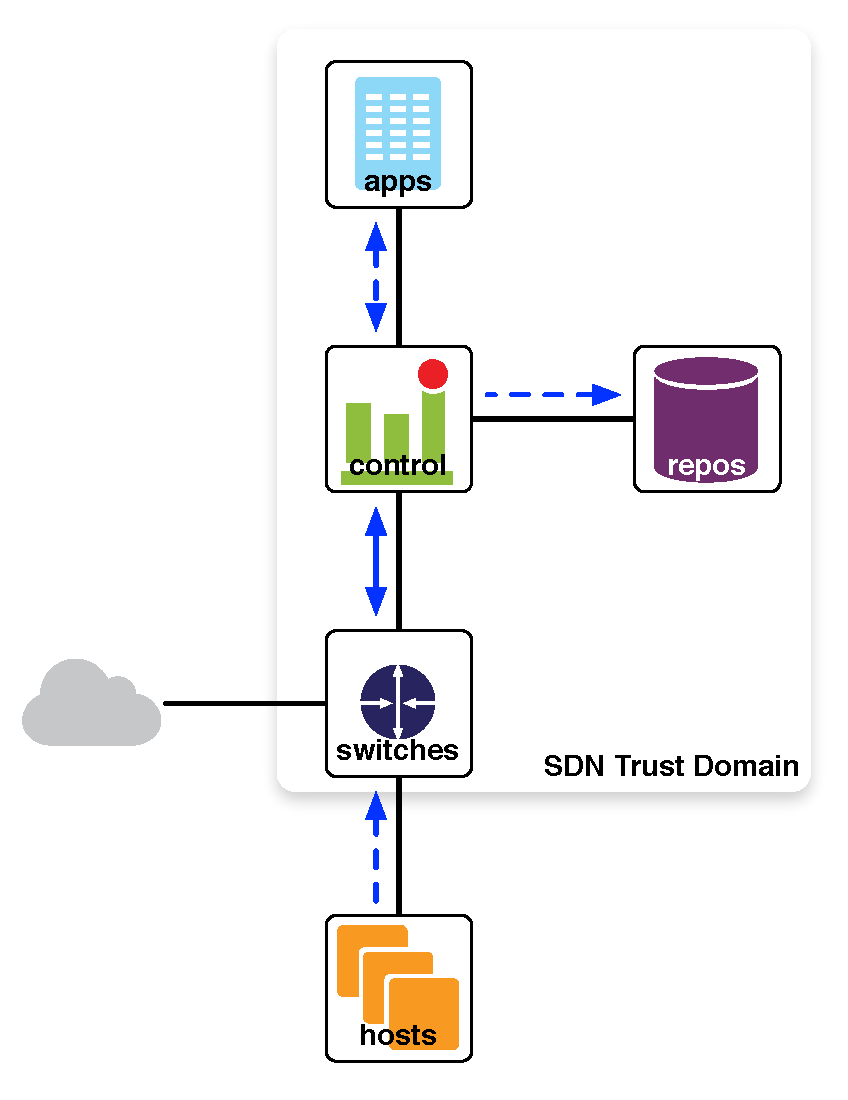
\includegraphics[height=2.75in]{reference-model}
\column{.5\textwidth}
So overall, how important are our typical cyber-security attributes?
\\~\\
\begin{beamerboxesrounded}[shadow]{}
\begin{itemize}
\item {\color{green} Confidentiality}
\item {\color{red} Integrity}
\item {\color{orange} Availability}
\item {\color{green} Non-repudiation}
\item {\color{red} Authentication}
\end{itemize}
\end{beamerboxesrounded}
\end{columns}
\end{frame}

\begin{frame}
\frametitle{Differentiating Attributes of SDN}
Compared to other more agent-centric systems, SDN control systems have some advantages:
\begin{itemize}
\item Limited control-plane volatility
	\begin{itemize}
	\item MANETs and agent-based systems are much more chaotic with respect to functional distribution (many devices wear multiple commmunication hats) and suffer from frequent attach / detach issues
	\end{itemize}
\item Centralized High-Availability
	\begin{itemize}
	\item Any high-availability requirements are constrained to specific functional areas (e.g. controllers)
	\end{itemize}
\item Clearly Defined Roles
	\begin{itemize}
	\item SDN entities have clear roles; systems in MANETs or agent-based systems frequently do not
	\end{itemize}
\item Predicable Expected Behavior
	\begin{itemize}
	\item Clear roles should lead to more predicable behavior and correspondingly easier behavioral outlier detection
	\end{itemize}
\end{itemize}
\end{frame}

\begin{frame}[c]
\begin{center}
\textbf{Questions? Comments?}
\end{center}
\end{frame}

\end{document}

